\documentclass[11pt]{standalone}

\usepackage{helvet}
\usepackage{units}
\usepackage{textcomp}

\usepackage{ifthen}
\usepackage{tikz} 
\usetikzlibrary{shapes.misc}
\usetikzlibrary{arrows,arrows.meta}
\usetikzlibrary{calc,intersections, patterns, math}
\usetikzlibrary{decorations.pathmorphing}
\usetikzlibrary{shapes.geometric}

\definecolor{pfeil}{RGB}{168,167,167}
\definecolor{petrol}{RGB}{0, 118, 136}
\definecolor{darkgoldenrod}{RGB}{184, 134, 11}
\colorlet{petrol-lighter}{petrol!40}
\colorlet{darkgoldenrod-lighter}{darkgoldenrod!40}

\newcommand{\polygon}[3]{ 
    % #1 = position
    % #2 = anzahl ecken
    % #3 = farbe 
    \pgfmathsetmacro{\MyRand}{3.6*random(0,100)}
    \node[#3, fill,regular polygon,draw,
	regular polygon sides = #2, rotate=\MyRand] at (#1) {\phantom{.}};
}

\begin{document}

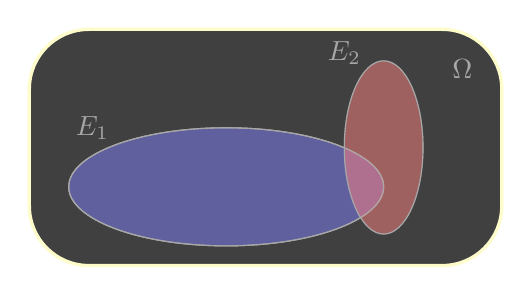
\begin{tikzpicture}[pfeil]

	\def\EllA{(2.5,1) ellipse (2 and 0.75)}
	\def\EllB{(4.5,1.5) ellipse (0.5 and 1.1)}


	% \draw[thick, fill=petrol!20, draw=petrol-lighter, rounded corners=2ex, opacity=0.5] (0,0) rectangle ++ (1.5,3.5);
	% \draw[thick, fill=darkgoldenrod!20, draw=darkgoldenrod-lighter, rounded corners=2ex, opacity=0.5] (5,0) rectangle ++ (1.5,3.5);

	\draw[draw=yellow!20, fill=darkgray, rounded corners=5ex, very thick] (0,0) rectangle (6,3);
	\node at (5.5,2.5) {$\Omega$};
	\draw[fill=blue!50, opacity=0.5] \EllA;
	\draw \EllA;
	\node at (0.8,1.75) {$E_1$};
	\draw[fill=red!50, opacity=0.5] \EllB;
	\node at (4,2.7) {$E_2$};
	\draw \EllA \EllB;

	% \fill[green!50!black]  \EllA \EllB;
	% \node at (3.5,1.05) {$E_1\cup E_2$};





\end{tikzpicture}




\end{document}
